
\documentclass[12pt,a4paper,UTF8]{article}
\usepackage{ctex} % Chinese support
\usepackage{graphicx} % Insert images
\usepackage{listings} % Print source code
\usepackage[usenames,dvipsnames]{xcolor}
\usepackage{color} % Color support
\usepackage{float}
\usepackage{booktabs} % Professional table support
\usepackage{pdflscape} % Landscape pages support in PDF
\usepackage{hyperref} % Hypertext links support for cross-referencing
% \lstnewenvironment{cpp}{\lstset{language=cpp,
% 	basicstyle=\ttfamily\footnotesize,
% 	keywordstyle=\bfseries\color[rgb]{0, 0, 1},
% 	identifierstyle=\color[rgb]{0.5, 0.3, 0.1},
% 	stringstyle=\color[rgb]{0.6, 0.1, 0.1},
% 	commentstyle=\itshape\color[rgb]{0.05, 0.5, 0.05},
% 	backgroundcolor=\color[gray]{0.95},
% 	numbers=left,numbersep=5pt,numberstyle=\color[gray]{0.6},
% 	breaklines=true}}{}
\definecolor{mygreen}{rgb}{0,0.6,0}
\definecolor{mygray}{rgb}{0.5,0.5,0.5}
\definecolor{mymauve}{rgb}{0.58,0,0.82}
\lstset{
 backgroundcolor=\color{lightgray}, 
 basicstyle = \footnotesize,       
 breakatwhitespace = false,        
 breaklines = true,                 
 captionpos = b,                    
 commentstyle = \color{mygreen}\bfseries,
 extendedchars = false,             
 frame =shadowbox, 
 framerule=0.5pt,
 keepspaces=true,
 keywordstyle=\color{blue}\bfseries, % keyword style
 language = C++,                     % the language of code
 otherkeywords={string}, 
 numbers=left, 
 numbersep=5pt,
 numberstyle=\tiny\color{mygray},
 rulecolor=\color{black},         
 showspaces=false,  
 showstringspaces=false, 
 showtabs=false,    
 stepnumber=1,         
 stringstyle=\color{mymauve},        % string literal style
 tabsize=2,          
 title=\lstname                      
}

% Customize hyperref format (it's set to no special format here)
\hypersetup{hidelinks}

% Declare directories to search for graphics files for graphicx
\graphicspath{{figures/}{logo/}}


% Define source code style for listings
\lstdefinestyle{verilog}{
  language=Verilog,
  basicstyle=\ttfamily\footnotesize,
  keywordstyle=\bfseries\color[rgb]{0, 0, 1},
  identifierstyle=\color[rgb]{0.3, 0.2, 0},
  stringstyle=\color[rgb]{0.6, 0.1, 0.1},
  commentstyle=\itshape\color[rgb]{0.05, 0.5, 0.05},
  backgroundcolor=\color[gray]{0.98},
  numbers=left,
  numbersep=5pt,
  numberstyle=\color[gray]{0.6},
  breaklines=true
}

% Define source code style for listings
\lstdefinestyle{cpp-style}{
  language=C++,
  basicstyle=\ttfamily\footnotesize,
  keywordstyle=\bfseries\color[rgb]{0, 0, 1},
  identifierstyle=\color[rgb]{0.5, 0.3, 0.1},
  stringstyle=\color[rgb]{0.6, 0.1, 0.1},
  commentstyle=\itshape\color[rgb]{0.05, 0.5, 0.05},
  backgroundcolor=\color[gray]{0.95},
  numbers=left,
  numbersep=5pt,
  numberstyle=\color[gray]{0.6},
  breaklines=true
}

% Define new command for title page
\newcommand{\reporttitle}[2]{
  \LARGE\textsf{#1}\quad\underline{\makebox[12em]{#2}}
}
\newcommand{\reportinfo}[2]{
  \large\makebox[4em]{\textsf{#1}}\quad\underline{\makebox[18em]{#2}}
}
% The document begins here
\begin{document}
  \begin{titlepage}
    \centering
    
    
\includegraphics[height=144pt]{figure/picture.png}\\[48pt] % Change the school logo here (See the logo/ directory) and adjust the height
    {\huge\textsf{植\ 物\ 大\ 战\ 僵\ 尸}}\\[48pt]
    \reporttitle{报告名称}{PVZ设计}\\[72pt]

    \reportinfo{课程名称}{高级程序设计}\\[8pt]
    \reportinfo{学生姓名}{时欣}\\[10pt]
    \reportinfo{学\hspace{\fill}号}{191220097}\\[8pt]
    \reportinfo{实验日期}{2021年5月5日}\\
        \vspace*{\fill}
  \end{titlepage}

  \tableofcontents
  \newpage

  \section{实验内容}
    实现一个升级版的植物大战僵尸,主要内容包括:
    \subsection{界面显示}
        \begin{enumerate}
          \item 3行7列的地块;
          \item 商店内容的显示;
          \item 计分表分值;
          \item 阳光拥有值的显示
          \item 光标显示————用于进入商店时,移动光标来选择购买的植物;确定购买后,移动光标来选择植物存放的地块,并在相应的地块显示植物;(除了种植的确认)如果确定
          后又取消("x"),则再次显示光标,重复以上步骤。
          \item 植物和僵尸的种类与生命值显示。其中每个地块可以有多个僵尸
        \end{enumerate}

    \subsection{游戏主体}
        \begin{enumerate}
          \item 僵尸:普通僵尸,路障僵尸,读报僵尸,撑杆僵尸,小丑僵尸,投石僵尸;
          \item 植物:豌豆射手,双发射手,寒冰射手,坚果墙,高坚果,窝瓜,樱桃炸弹,大蒜,南瓜头;
          \item 攻击工具:普通子弹,寒冰射手的子弹;
        \end{enumerate}

    \subsection{游戏逻辑}
        \begin{enumerate}
          \item 塔防逻辑:植物有其对应的生命值和攻击力(每秒对僵尸造成多少伤害),僵尸有其对应的生命值,攻击力(每秒对植物造成多少伤害)和速度(走到
          下一个地块需要多少秒)。\\
                        当僵尸走到植物所在地块时可以对植物进行攻击;当植物的生命值减到0则植物死亡,从植物列表中移除,而僵尸可以走到下一个地
            块对其中的植物攻击。如果僵尸将最左侧地块的植物攻击致死,则游戏失败。\\
            其中对于植物
          \begin{enumerate}
            \item 豌豆射手、双发射手和寒冰射手的作用是每秒发射子弹,真正起作用的是子弹。子弹有其伤害值(一个子弹对僵尸造成多少伤害)和速度,当子弹与僵尸在同一个地块时,
            子弹对僵尸造成伤害,随后子弹消亡。当僵尸的生命值减到0则僵尸死亡。而寒冰射手的子弹还会让僵尸减速。
            \item 大蒜的作用是当其生命值减少时,对应给它造成伤害的僵尸会到相邻的地块中。
            \item 坚果墙和高坚果都没有攻击功能,只能在其还存活时对僵尸造成阻挡作用。
            \item 窝瓜的作用是当僵尸走到有它的地块,则使僵尸死亡并且自身死亡。
            \item 樱桃炸弹的作用是以自己为中心3*3范围内的僵尸死亡并且自身死亡。
            \item 南瓜头所在地块如果有其他植物,则南瓜头先收到攻击。
          \end{enumerate}
          而对于僵尸
          \begin{enumerate}
            \item  移动逻辑中,只有撑杆僵尸和投石僵尸由于自身的性质具有特殊性。撑杆僵尸是在有杆的时候能够跨越除了高坚果以外的植物,没有杆的时候和普通僵尸一样;而投石僵尸是
            在有石头并且左边有植物的时候原地不动,除此之外,正常移动。其他僵尸的移动逻辑都和普通僵尸一样。
            \item 普通僵尸只有当所在地块有植物时对它进行攻击,撑杆僵尸也是。\\
                  路障僵尸和普通僵尸的攻击逻辑相同,只是生命值更高。\\
                  读报僵尸和普通僵尸的攻击逻辑相同,只是受到攻击后速度会加快。\\
                  小丑僵尸在10\%的情况下会自爆,炸毁以自身为中心3*3地块的植物,90\%的情况下攻击逻辑和普通僵尸相同。\\
                  投石僵尸在有石头并且这一排有植物的时候会对左边的植物进行石头的攻击。在没有石头的时候,会直接造成所到地块植物的死亡。\\
          \end{enumerate}

          \item 购买逻辑:植物有其对应的阳光消耗值,选定购买以后,阳光拥有值扣除相应的数量。如果阳光拥有值不足,则无法购买,对用户给出提示。如果冷却时间不够,则无法购买,对
          用户给出提示。
          \item 种植逻辑:如果当前地块没有种植植物或者只种了南瓜头,则可以种植。否则不能种植。
          
        \end{enumerate}
    

\section{实验目标}
    实现较好的交互界面,完成游戏正确的逻辑,丰富植物和僵尸的种类。

\section{实验环境}
\begin{enumerate}
  \item 设计语言:c++
  \item 运行环境:Windows
  \item 设计环境:Visual Studio 2019
\end{enumerate}
  
\section{实验设计思路}
    运用c++语言,运用面向对象的思路设计。
    \begin{enumerate}
      \item 需要实现的各类间关系如下图
          \begin{figure}[H]
            \centering
          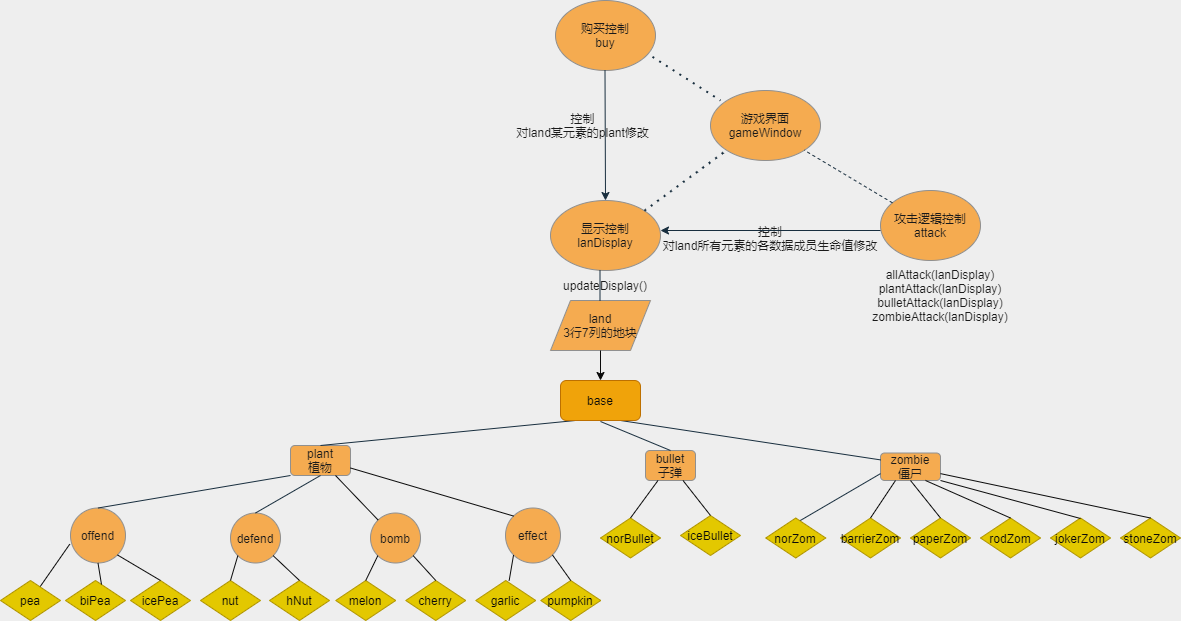
\includegraphics[width=0.9\textwidth]{figure/UMI.png}
          \caption{各类间关系}
          \end{figure}
        图中的各个图形标出的都是一个类(除了UI模块)。zombie,bullet,plant由基类base派生而来,而具体的植物、子弹和僵尸类型由它们派生而来。land控制三个数组,即存放僵尸,子弹和
        植物的数组,而land由lanDisplay控制。
    \item 设计思路\\
        如上图所示,lanDisplay类下有一个land类成员,而land类下有上述的三个数组成员。采用类对象直接通信的机制。即lanDisplay类一旦发现zombie,bullet,plant发出的信号,
        即这三个类对lanDisplay发送消息————我要移动了,或者我要攻击了。然后lanDisplay来控制,经过判断以后看能不能允许它们移动或者攻击。也就是
        能对地块状态进行改动的只有lanDisplay类,如果其它的类想要对地块状态进行改动,只能给lanDisplay发消息,通过lanDisplay来仲裁能否改动。\\
        而对于程序显示和定时刷新,我选择的是,每一轮攻击之后使用Sleep函数让程序休眠500ms,再继续,这样每一轮的输出都会停顿一下,以实现视觉上的动态变化效果。每一轮刷新,UI模块会
        读取lanDisplay的状态来输出。\\
        最后在main函数里面调用函数实行整个游戏的逻辑————用一个while循环,在游戏未失败的情况下,反复执行一轮一轮的攻击与移动。并且每当一段时间之后利用random随机选择一行产生僵尸,
        以及每当一段时间之后对系统阳光增加50。
    \end{enumerate}

\section{各个类的设计}
    \subsection{zombie类}
      \begin{figure}[H]
        \centering
      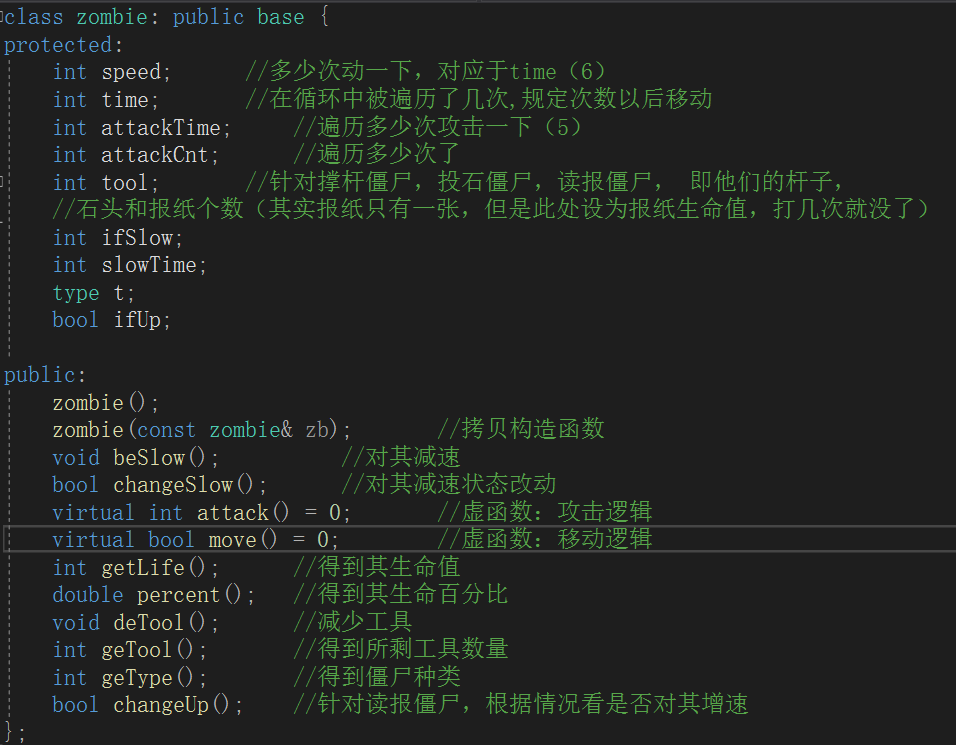
\includegraphics[width=0.7\textwidth]{figure/zombie.png}
      \caption{zombie类数据与操作}
    \end{figure}
      各个数据成员与成员函数的含义如注释所标。之所以要实现拷贝构造函数是因为,僵尸移动时需要带着它的状态(生命值等)走,也就是需要先在原先的
      地块删掉它, 然后在下一个地块新建一个和它一样的对象。
      如果被寒冰射手打中,那么减速时间持续五次遍历的时间,所以需要在每次遍历的时候对遍历次数的计数做额外处理。我没有另外写一个函数,而是直接放在僵尸的move里面了,也就是在判断
      完是否还活着以后,直接根据是否在减速的状态,就对其的计数做操作。

      僵尸的攻击比较复杂,采用虚函数和动态绑定,针对不同的情况给总控制类发出不同的返回值信号来显示自己需要干什么
      注意有道具的僵尸,需要判断其道具的存在性
      而其中对于move来说
      \begin{enumerate}
        \item 撑杆僵尸: 它的move应该首先判断左边一格是否有植物并且此植物并非高坚果,如果true那么就向控制类发出信号1————表示请求跳过左侧植物;如果false,那么对遍历次数计数,
        和普通僵尸一样,到次数移动
        \begin{figure}[H]
          \centering
        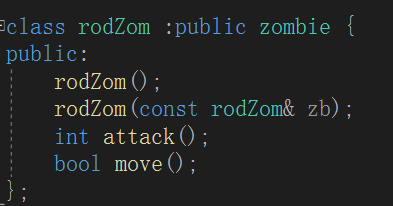
\includegraphics[width=0.6\textwidth]{figure/rodZom.png}
        \caption{rodZom类数据与操作}
      \end{figure}
        \item 投石僵尸:它的move需要判断石头有没有扔完石头,如果扔完了又到了移动的时候,那么就往左走。如果没有扔完但是左边没有任何植物,那么它也会往左走。
        额外增添了是否扔石头的两个变量stoneCnt和stoneTime
        \begin{figure}[H]
          \centering
        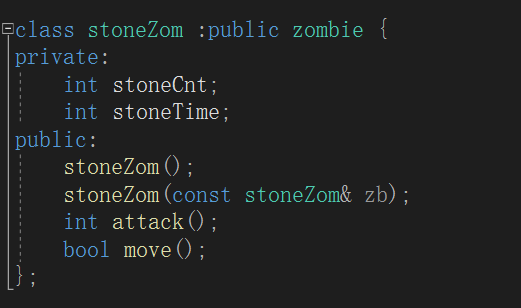
\includegraphics[width=0.6\textwidth]{figure/stoneZom.png}
        \caption{stoneZom类数据与操作}
      \end{figure}
        \item 读报僵尸:它的move和普通僵尸一样,但是需要注意,当其受到伤害时应当使用changeUp函数对其速度进行改动
        \begin{figure}[H]
          \centering
        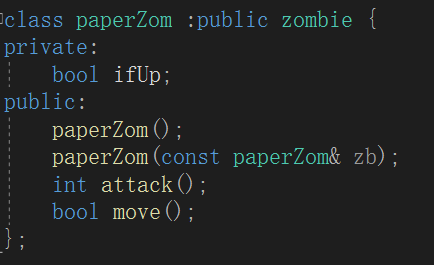
\includegraphics[width=0.7\textwidth]{figure/paperZom.png}
        \caption{paperZom类数据与操作}
        \end{figure}
        \item 路障僵尸和小丑僵尸:move和普通僵尸一样。额外增添了ifUp变量,用来判断是否已经没有报纸从而加速
        \begin{figure}[H]
          \centering
        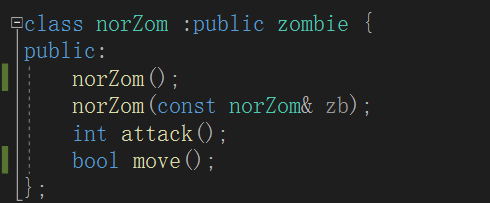
\includegraphics[width=0.7\textwidth]{figure/norZom.png}
        \caption{norZom类数据与操作}
        \end{figure}
        路障僵尸和小丑僵尸的具体操作就不再额外给出
        
      \end{enumerate}
      其中对于attack来说
      \begin{enumerate}
        \item 撑杆僵尸:它的attack是和普通僵尸一样(其实只有在面对高坚果的时候有效)
        \item 投石僵尸:它的attack是首先需要判断还有没有石头。如果有,那么到扔石头的时候,就告诉控制类要攻击植物了(从它的位置开始往左遍历,攻击最近的僵尸)。如果没有,就和普通僵尸
        一样,当前地块上有植物的话就让植物死亡
        \item 读报僵尸和路障僵尸:和普通僵尸一样
        \item 小丑僵尸:首先会有一个概率得出它要不要爆炸,如果不爆炸就和普通僵尸一样。如果爆炸就将周围3*3的植物都生命值置零。
      \end{enumerate}
      其中定时攻击的逻辑如下(以路障僵尸为例)
      \begin{figure}[H]
        \centering
      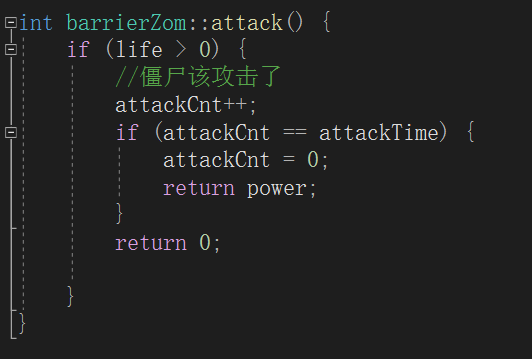
\includegraphics[width=0.7\textwidth]{figure/zomAttack.png}
      \caption{僵尸定时攻击}
      \end{figure}
      如果僵尸的attackCnt的值已经和attackTime的值相等,则僵尸可以对植物发动攻击,对应的植物扣除相应的生命值。否则attackCnt的值加1————以此来实现僵尸对植物的定时攻击。
      
      此处给出ifSlow的实现
      \begin{figure}[H]
        \centering
      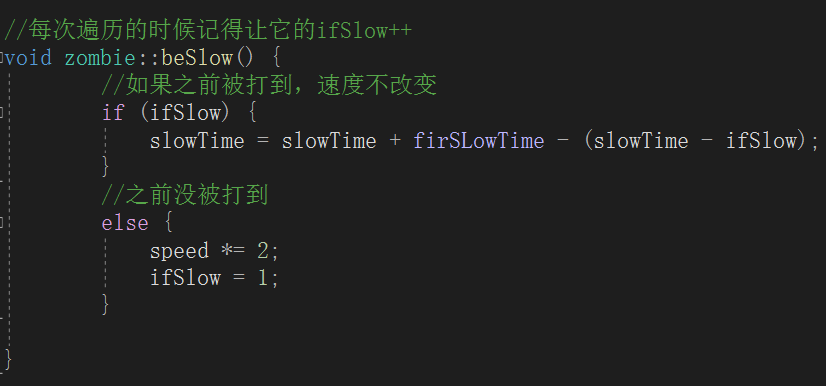
\includegraphics[width=0.65\textwidth]{figure/ifSlow.png}
      \caption{ifSlow逻辑展示}
      \end{figure}
      需要注意如果一个僵尸上一次的减速还未结束,又别打中,并不是简单的进行减速时间叠加,而是需要减去重叠部分。

    \subsection{plant类}
      \begin{figure}[H]
        \centering
      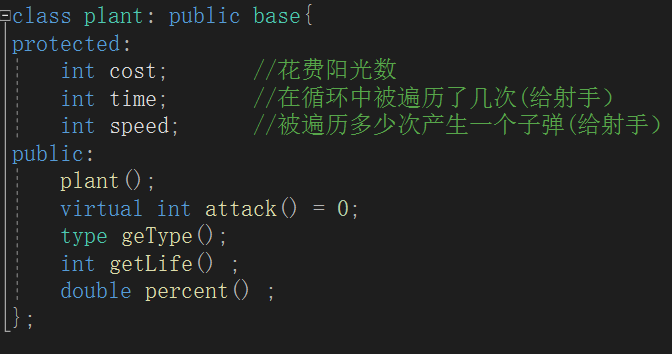
\includegraphics[width=0.65\textwidth]{figure/plant.png}
      \caption{plant类数据与操作}
      \end{figure}
      各个数据成员与成员函数的含义如注释所标。需要实现默认构造函数,得到植物的类型,生命值,生命值比例的函数\\
      而从它继承下来的类,函数也就是自己的默认构造函数和attack虚函数的实例化,所以此处不再额外给出图\\
      具体写一下attack函数的实现,以寒冰射手的attack为例
      \begin{figure}[H]
        \centering
      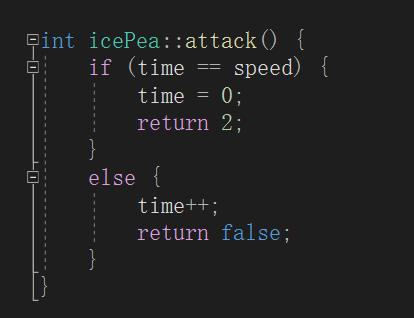
\includegraphics[width=0.6\textwidth]{figure/attack.png}
      \caption{attack逻辑展示}
      \end{figure}
      如上图,time==speed即判断是否到了攻击的时间,其实射手本身是不能对僵尸发动攻击的,因此它的攻击其实就是定时产生子弹。每一次遍历,如果发现time的值已经和speed的值相等
      则令射手产生子弹,否则time的值加一————以此来模拟射手的定时发射子弹。而返回的值表示着不同的植物类型,如果返回值为0则没到攻击的时候,如果不为0会根据植物类型的不同返回
      不同的值,让控制类知道根据植物类型应该做什么。


    \subsection{bullet类}
    \begin{figure}[H]
      \centering
    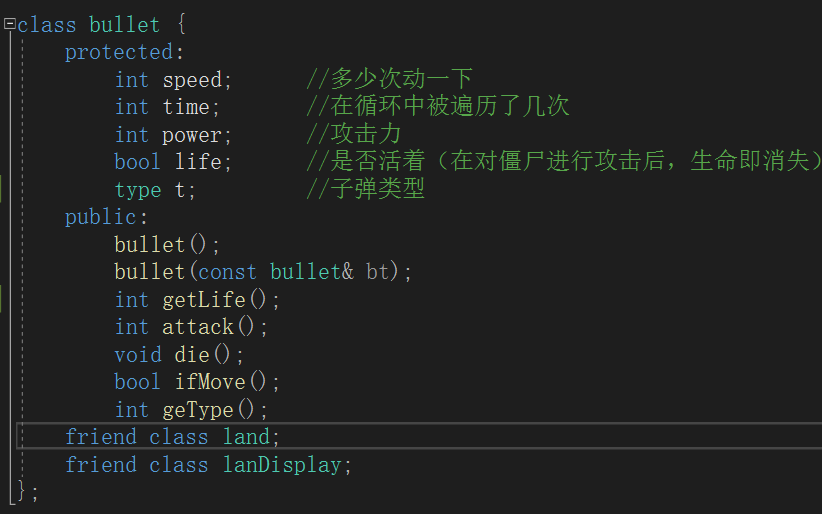
\includegraphics[width=0.6\textwidth]{figure/bullet.png}
    \caption{bullet类数据与操作}
    \end{figure}
    各个数据成员与成员函数的含义如注释所标。比较简单,不再赘述。

    \subsection{land类}
      \begin{figure}[H]
        \centering
      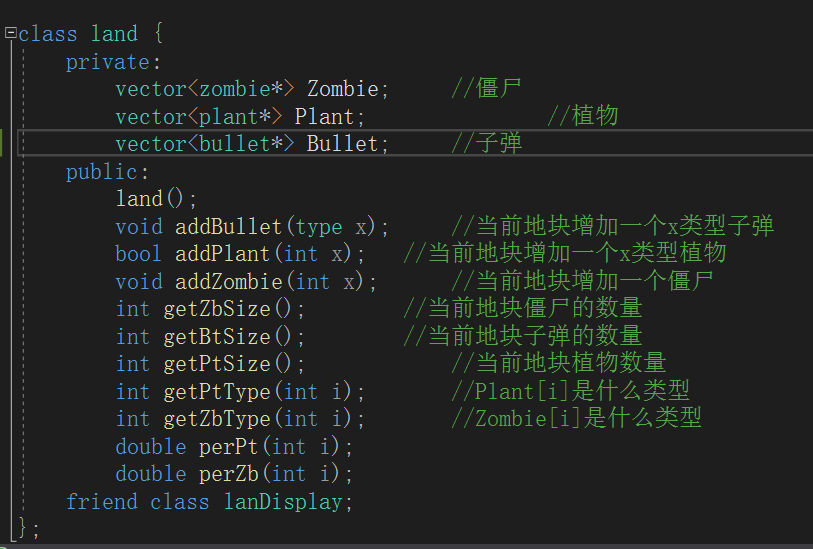
\includegraphics[width=0.6\textwidth]{figure/land.png}
      \caption{land类数据与操作}
      \end{figure}
      各个数据成员与成员函数的含义如注释所标。每一个land类的对象都是一块地块,各自管理各自的有关植物、僵尸和子弹的状态。\\
      而之所以数组要使用指针类型,是为了之后的动态绑定,根据植物、子弹和僵尸类型的不同,调用attack等虚函数时可以绑定到具体那一种类型的attack上面。

    \subsection{lanDisplay类}
    \begin{figure}[H]
      \centering
    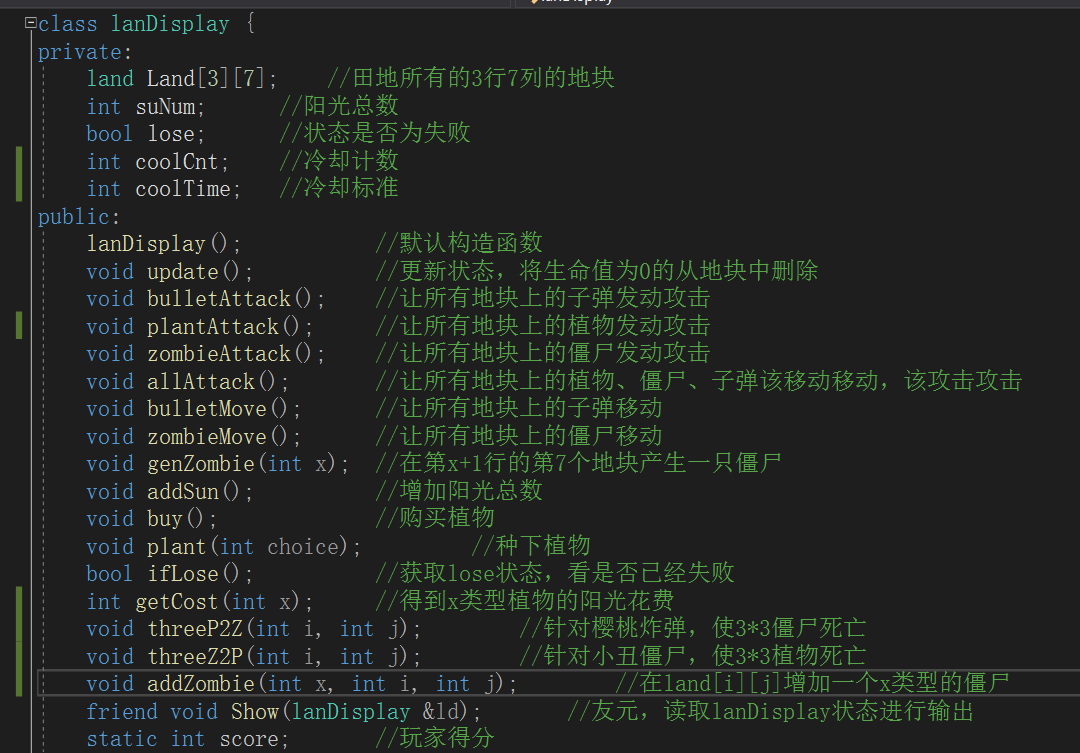
\includegraphics[width=0.7\textwidth]{figure/lanDis.png}
    \end{figure}
    \begin{enumerate}
      \item 各个数据成员与成员函数的含义如注释所标。lanDisplay类作为整个设计的核心控制类在本程序中占有极其重要的地位。
      \item 可以看到lanDisplay类中有数据成员land Land[3][7],即将所有地块以二维数组的形式进行组织,各个地块中又存储着属于自己的有关植物、僵尸和子弹的状态。
      \item 而lanDisplay类是land、植物、僵尸和子弹类的友元,因此通过lanDisplay类可以对地块的各种状态进行改动,从而实现对于地块中各个游戏主题的移动和攻击逻辑进行控制。
      \item lanDisplay类中的成员函数bulletAttack();是通过对于Land[3][7]中的每一个地块中的bullet成员进行遍历来实现的。
      每一次遍历,如果发现子弹所在地块有僵尸,则僵尸被扣除子弹攻击一次会产生的伤害值,然后将子弹的生命值置零。而其中如果是寒冰射手还会令僵尸的速度减半
      \item plantAttack();也是通过对于Land[3][7]中的每一个植物进行遍历来实现的。根据各自attack函数的返回值,决定是否攻击,进行怎样的攻击。\\
      因此会有分支语句,根据不同植物的特性做出相应的攻击。由于具体的攻击比如使得僵尸全部死亡等等,这些实现非常简单,就不必赘述了。主要还是这个框架思路比较重要。
      \item zombieAttack();是通过对于Land[3][7]中的每一个地块中的zombie成员进行遍历来实现的。攻击逻辑为:在当前地块有僵尸且其生命值大于0,并且当前地块有植物且其生命值大于
      0的情况下,根据其attack的返回值决定要不要进行攻击以及进行怎样的攻击。\\
      而相比较第一次,由于僵尸的种类变多了,有些僵尸需要进行特殊操作,所以这个函数时有改动的。\\
      注意大蒜的攻击逻辑实际上是在这里实现的————即对植物造成伤害后,会判断这个植物是不是大蒜,如果是则会对僵尸的位置进行改动。
      \item bulletMove()是通过对于Land[3][7]中的每一个地块中的bullet成员进行遍历来实现的。如果当前地块没有僵尸,且子弹已经到了其该移动的时候(通过调用ifMove函数得到
      其是否要移动的信息。如果要移动,则在下一个地块新建一个bullet,把当前地块的bullet删除。\\
      当然,如果已经在最后一个地块了,那么直接将其删除即可。当然,如果当前地块有僵尸,那么它暂时不能移动,因为接下来它需要对僵尸进行攻击。
      \item zombieMove()是通过对于Land[3][7]中的每一个地块中的zombie成员进行遍历来实现的。如果当前地块没有植物,并且僵尸已经给出了要移动的信号,则根据僵尸的不同特性进行
      移动(强调这一点是因为撑杆僵尸和投石僵尸的特殊性)。如果只是普通僵尸,那么将当前地块的僵尸拷贝到下一个地块,将当前地块的僵尸删除。\\
      需要注意,如果僵尸已经在最左边的地块而且也没有植物了,那么僵尸越过这个地块以后lanDisplay的lose状态将会被置为1,也就是说玩家失败。
      \item 额外说的一点是————为了实现在一个地块有南瓜头和另一个植物的逻辑。如果插入南瓜头,会把它放到plant数组的首个位置,这样僵尸攻击是按序遍历数组的,就会先攻击南瓜头。
    \end{enumerate}
    总的来说,lanDisplay类是通过与zombie,bullet,plant的通信来控制地块状态的,一旦得到他们的信号————我要移动了,或者我要攻击了。
    则lanDisplay来进行判断,看能不能允许它移动或者攻击。
    \begin{enumerate}
      \item 而update函数则是对地块状态进行更新,主要是全部遍历,将生命值为0的游戏主体从地块中删除,并且根据lose状态判断玩家是否失败
      来决定是否游戏结束。
      \item buy函数和plant函数本来是想放在lanDisplay类外面,单独作为一个类并和lanDisplay类交互的。可是因为是直接对lanDisplay中的地块状态进行操作,所以干脆放在了一个类里面。
      通过查阅资料,我知道了如何获取键码。\\
      我是通过光标的停留位置来判断用户的选择的。用户可以通过按下wasd键等来移动光标位置,y和enter来确认选择,x来取消。对地块的状态改动,是发生在
      选择好植物并确认种植以后,一旦获取到相应的键码,则在对应的地块上增加用户选择的植物。(当然如果判断到键码但发现阳光总数不够,则不会对地块进行改动,而是在界面下方对用户进行提示。\\
      相关代码为
      \lstinputlisting[style=verilog]{mouse.cpp}
      先判断是否有按键按下,如果有,获取键码,根据键码做相应事件。从买到种植,如果中间没有取消工作,是一个顺序循环读取键码的过程,所以采用while循环。\\
      注意相比较第一次,多了一个冷却时间的功能。也就是通过lanDisplay新增加的成员coolCnt和coolTime实现的,如果成功购买并且种植了一个植物,那么冷却计数开始,每次计数+1,最后
      冷却计数到达可以停止的时候,则可以再次购买植物,否则对玩家进行提示
    \end{enumerate}

  
    
\section{程序亮点}
\begin{enumerate}
  \item 选择用一个类实现总控制的方法,模仿各个进程给操作系统发信息请求资源调度等让操作系统仲裁决定的方式,让其它类都给lanDisplay类发送自己的状态,而lanDisplay类接收到信息以后
  做出判断和相应操作。
  \item UI和游戏逻辑分离,只读取lanDisplay状态进行输出,不做别的多余的动作。
  \item 利用了继承和动态绑定,大大减小了代码量,实现了代码冗余的改善。且继承的层次关系分明。
  \item 实现了很好的封装性,friend友元的使用极少,很好的保护了类的成员私密性。主要通过接口和外界交互。
  \item 游戏界面更加稳定,不闪烁。
  相比较上次是每次刷新都会清屏,导致会特别闪,用户体验很不好。为了改善,选择了每次都会先输出背景(即整个田地即商店得分等的背景),然后再得到输出位置从而一个一个地块的进行相应的
  输出的方式。成功实现了比较顺畅的游戏体验。且为了让子弹和僵尸植物不互相覆盖,开始输出的位置不太一样,从而即使重叠也可以看到一部分。
  \item 游戏有主界面,当前有两个选项,如下图
  \begin{figure}[H]
    \centering
  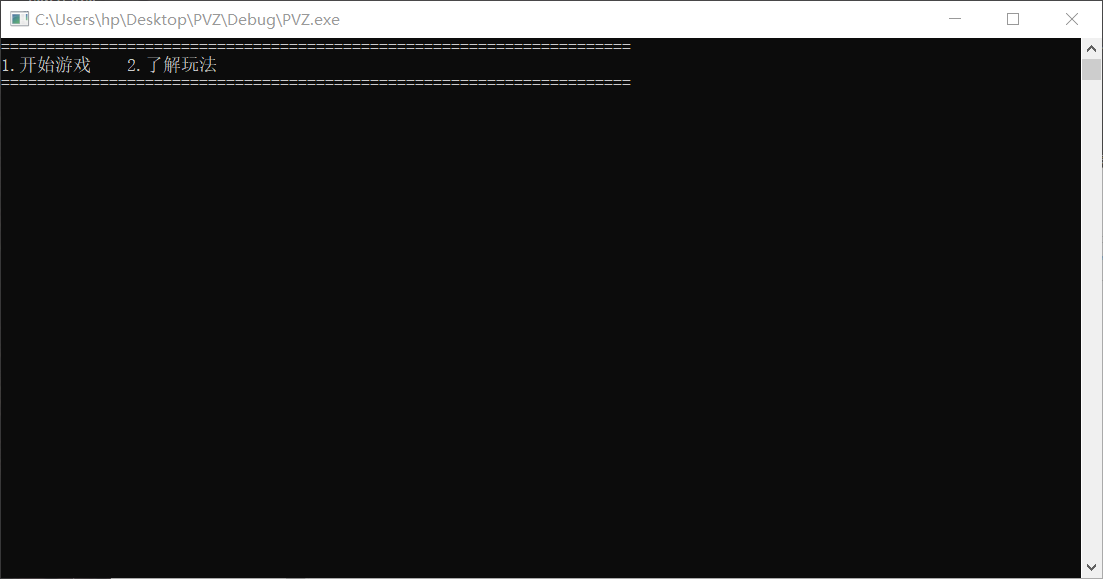
\includegraphics[width=0.7\textwidth]{figure/main.png}
  \caption{主界面}
  \end{figure}
  选择1则进入游戏界面,如下图(不同的颜色更加醒目)
  \begin{figure}[H]
    \centering
  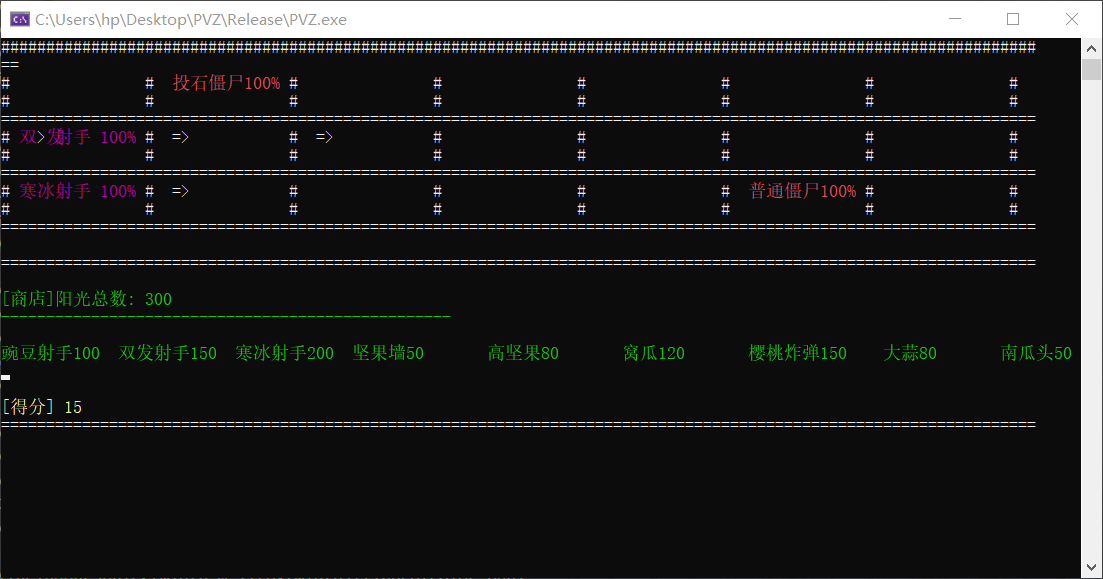
\includegraphics[width=0.7\textwidth]{figure/game.png}
  \caption{游戏界面}
\end{figure}
  选择2则进入游戏玩法说明,如下图
  \begin{figure}[H]
    \centering
  
\includegraphics[width=0.7\textwidth]{figure/rule.png}
  \caption{游戏规则}
  \end{figure}
  \item 对用户友好,如果阳光购买植物时不足、不能种植,或未到会给出提示
  \begin{figure}[H]
    \centering
  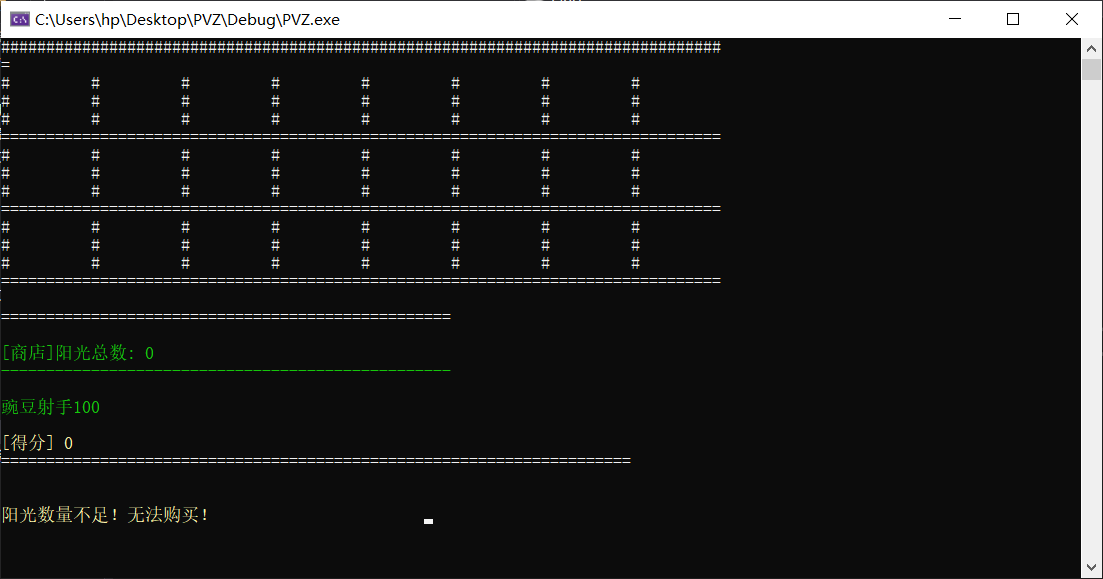
\includegraphics[width=0.7\textwidth]{figure/cout.png}\\
  \caption{提示如最后一行}
  \end{figure}
 
  如果中途购买或种植时选择错误,可以按下“x”取消。
  如果用户游戏失败,会有一个持续1s的“游戏失败”提示,然后返回主界面,进行下一轮新的游戏。
  如果用户在已种植植物的地块上选择种植新的植物,会在游戏界面下方提示,并且可以重新选择。
\end{enumerate}
      
    
  
\section{玩法}
  \subsection{游戏开始界面}
  \begin{enumerate}
    \item 选择开始游戏则进入游戏界面
    \item 选择了解玩法,则显示游戏规则;按下enter则返回主界面。
  \end{enumerate}
  
  \subsection{商店购买规则}
  \begin{enumerate}
      \item 玩家可以通过按下"b"来选择需要购买的植物,按下"b"后,商店中对应的植物下方会出现光标,玩家在光标出现在想买植物下方时按下"y"键即可获得出现在地块上的光标进行种植。如果选择了
      并不存在的植物则无效。按下“x”键可以取消购买。
      \item 当光标在地块中显示时,玩家可以通过按下"w""s""a""d"表示上下左右,来移动,当光标出现在想选择的地块内时,按下“enter”即可在对应地块种下相应植物。按下“enter”后无法取消
      种植行为,而在这之前如果按下"x"可以回到商店选择界面。
      \item 商店会显示对应植物购买所需的阳光数,如果显示的阳光总数足够则可以进行购买;如果阳光不足,那么会在界面下方对用户进行提示
  \end{enumerate}

  \subsection{攻击规则}
  \begin{enumerate}
    \item 一共有3行7列地块。僵尸会随机出现在某一行的最右侧地块。玩家需购买植物来守卫自己的家(在游戏界面的最左边)。购买货币为阳光,由系统定时生成,总数显示在界面下方。
    \item 现有植物为豌豆射手,其功能为定时产生子弹。当子弹打到僵尸时,对僵尸造成定量伤害,随后这颗子弹被消耗。如果僵尸走到植物所在的地块,那么僵尸可以对植物进行攻击,直到植物被僵尸伤害至生命值
    为0,僵尸才可以走到下一个地块。
    \item 如果僵尸走到了最左边的地块(即家所在的最后一道防线),且地块上的植物被攻击致死,那么僵尸到达了“家”,玩家游戏失败。
  \end{enumerate}

  \subsection{计分规则说明}
    每打死一只僵尸,总分加五分。游戏为无尽模式,因此,只要僵尸并未攻击到“家”,则积分一直累计。

\subsection{总结与感想}
这次对代码做了很大改动,把很大一部分lanDisplay判断的信号放到了具体植物子弹僵尸类的内部实现,而给总控制类的信号仅为一个函数的返回值。\\
并且调整了游戏界面,相比较第一次,僵尸、植物和子弹不在一行,这一版本更接近原版,是的僵尸子弹和植物在一行,其中南瓜头会另外实现。其实游戏界面的调整还挺痛苦的,出了很多很多问题,
也是打断点一点一点的看,发现哪里出问题,再去改动。另外由于第一次的游戏界面实在太闪了,我觉得可能没人想玩这种令人眼瞎的游戏。。。所以做了很多尝试,终于得到了目前这个版本的输出还算
稳定的界面。\\
另外一开始对继承和动态绑定使用的并不熟练,犯了很多错,也在debug的过程中把代码越写越多过,经过不断的尝试,尽可能的减少了代码量,并且对继承和动态绑定的使用理解的跟深刻了。\\
总的来说,debug和重构的过程稍显痛苦,但最终实现的效果还是令人欣喜的。最后,感谢老师和学长们的辛苦付出!



%\lstinputlisting[style=verilog]{md5_inout.v}

      
  \end{document}



